\section{Технологическая часть}

В данном разделе будут рассмотрены детали реализации программного комплекса, описанного в конструкторской части работы, представлены листинги кода алгоритмов обработки изображений и приведены примеры работы программы.

\subsection{Требования к программе}

Программа должна предоставлять следующие возможности:

\begin{enumerate}[leftmargin=1.6\parindent]
	\item[---] отображение загруженного изображения, а также результатов его обработки;
	\item[---] применение фильтров к изображению;
	\item[---] настройка яркости и контрастности изображения;
	\item[---] поворот изображения на 90 градусов по и против часовой стрелки;
	\item[---] операции отмены и повторения отмененного действия;
	\item[---] сохранение изображения.
\end{enumerate}

\subsection{Выбор языка программирования и среды разработки}
Существует множество языков, а также сред программирования, многие из которых обладают достаточно высокой эффективностью, удобством
и простотой в использовании. Для разработки данной программы был выбран язык C++ \cite{cpp-lang}. Данный выбор был обусловен следующими факторами:

\begin{enumerate}[leftmargin=1.6\parindent]
	\item[1.] Этот язык предоставляет программисту широкие возможности реализации самых разнообразных алгоритмов. Он обладает высокой эффективностью и большим набором стандартных классов и процедур.
	\item[2.] Язык является объектно-ориентированным, что позволяет объединить всю логику обработки изображения в класс.
	\item[3.] Язык является строго типизированным, что позволяет защититься от
	неконтролируемых ошибок.
	\item[4.] В данном языке имеется большое количество библиотек и шаблонов,
	позволяющих не тратить время на изобретение готовых конструкций.
\end{enumerate}

В качестве среды разработки был выбран фреймворк Qt \cite{qt} в силу следующих факторов:

\begin{enumerate}[leftmargin=1.6\parindent]
	\item[---] широкие возможности работы с изображениями, в том числе и попиксельно;
	\item[---] наличие более функциональных аналогов стандартной библиотеки шаблонов в том числе для разнообразных структур данных;
	\item[---] возможность написать интерфейс для программы.
\end{enumerate}

\subsection{Реализация алгоритмов обработки изображений}

\subsubsection{Изменение яркости и контрастности изображения}

В листинге \ref{code:1} представлены алгоритмы изменения яркости и контрастности изображений.

\begin{code}
	\captionof{listing}{Изменение яркости и контрастности изображения}
	\label{code:1}
	\inputminted
	[
	frame=single,
	framerule=0.5pt,
	framesep=20pt,
	fontsize=\small,
	tabsize=4,
	linenos,
	numbersep=5pt,
	xleftmargin=10pt,
	]
	{text}
	{code/code1.cpp}
\end{code}

\subsubsection{Фильтры}

В листинге \ref{code:2} представлены алгоритмы фильтров негатива, оттенки серого, размытия и уменьшения шума.

\begin{code}
	\captionof{listing}{Фильтры}
	\label{code:2}
	\inputminted
	[
	frame=single,
	framerule=0.5pt,
	framesep=20pt,
	fontsize=\small,
	tabsize=4,
	linenos,
	numbersep=5pt,
	xleftmargin=10pt,
	]
	{text}
	{code/code2.cpp}
\end{code}

\subsection{Интерфейс программы}

Общий интерфейс программы выглядит следующим образом (рис. \ref{fig:spire31}).

\begin{figure}[hbtp]
	\centering
	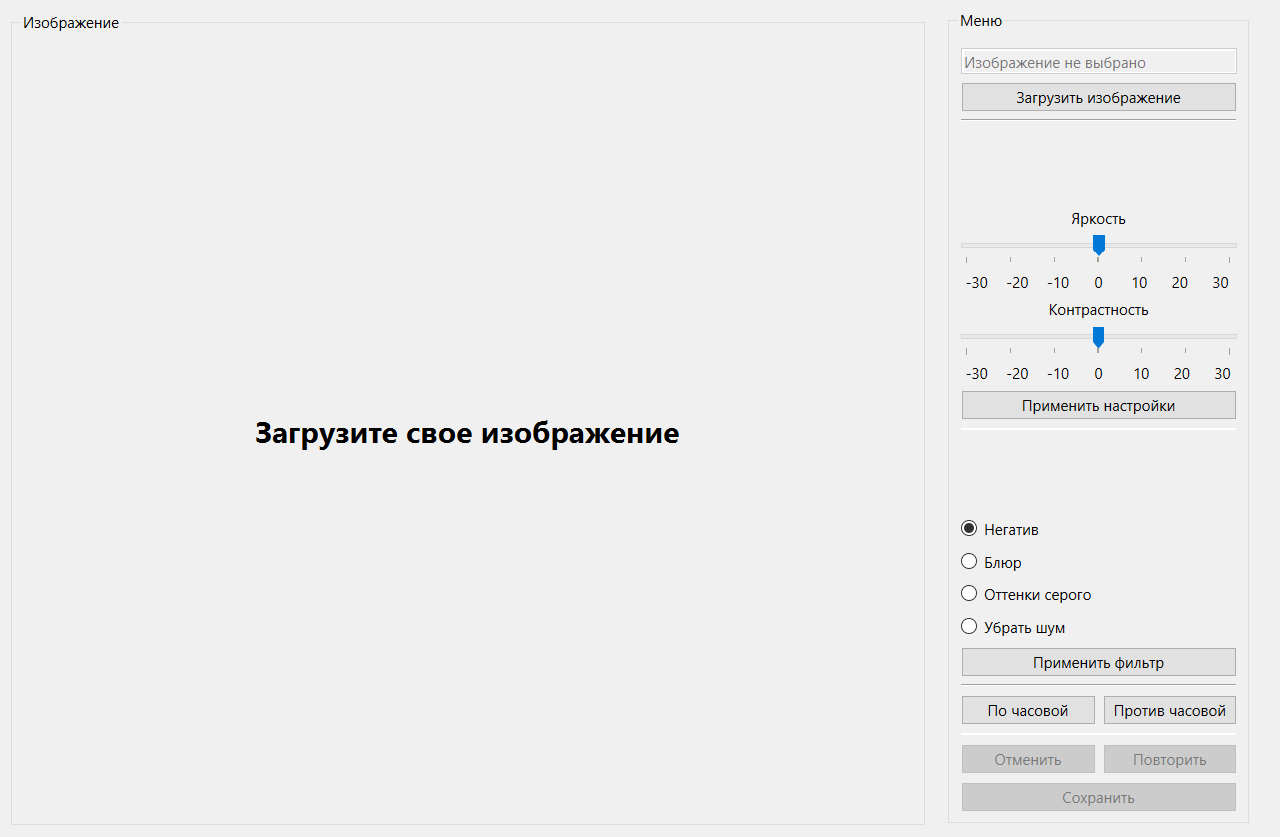
\includegraphics[width=0.9\textwidth]{img/res1.png}
	\caption{\label{fig:spire31} Интерфейс программы}
\end{figure}

Функции представленных кнопок следующие:

\begin{itemize}[leftmargin=1.6\parindent]
	\item[---] кнопка «Загрузить изображение» -- позволяет пользователю выбрать изображение с диск, которое в последствии будет обрабатываться;
	\item[---] слайдеры «Яркость» и «Контрастность» -- отвечают за одноименные параметры изображения;
	\item[---] кнопка «Применить настройки» -- считать значения со слайдеров «Яркость» и «Контрастность» и изменить параметры изображения на эти значения;
	\item[---] радиокнопки «Нетагив», «Блюр», «Оттенки серого» и «Убрать шум» -- отвечают за выбор фильтра;
	\item[---] кнопка «Применить фильтр» -- применяет выбранный фильтр к загруженному изображению;
	\item[---] кнопки «По часовой» и «Против часовой» -- вращают изображение по или против часовой стрелки соответственно;
	\item[---] кнопки «Отменить» и «Повторить» -- отвечают за историю преобразований, первая отменяет предыдущее действие, а вторая повторяет последнее отмененное действие;
	\item[---] кнопка «Сохранить» -- сохраняет результат обработки на диск.
\end{itemize}

\subsection{Демонстрация работы программы}

На рисунках \ref{fig:spire32}, \ref{fig:spire33}, \ref{fig:spire34} и \ref{fig:spire35} показаны результаты применения фильтров негатива, размытия, оттенков серого и уменьшения шума соответственно.

\begin{figure}[hbtp]
	\centering
	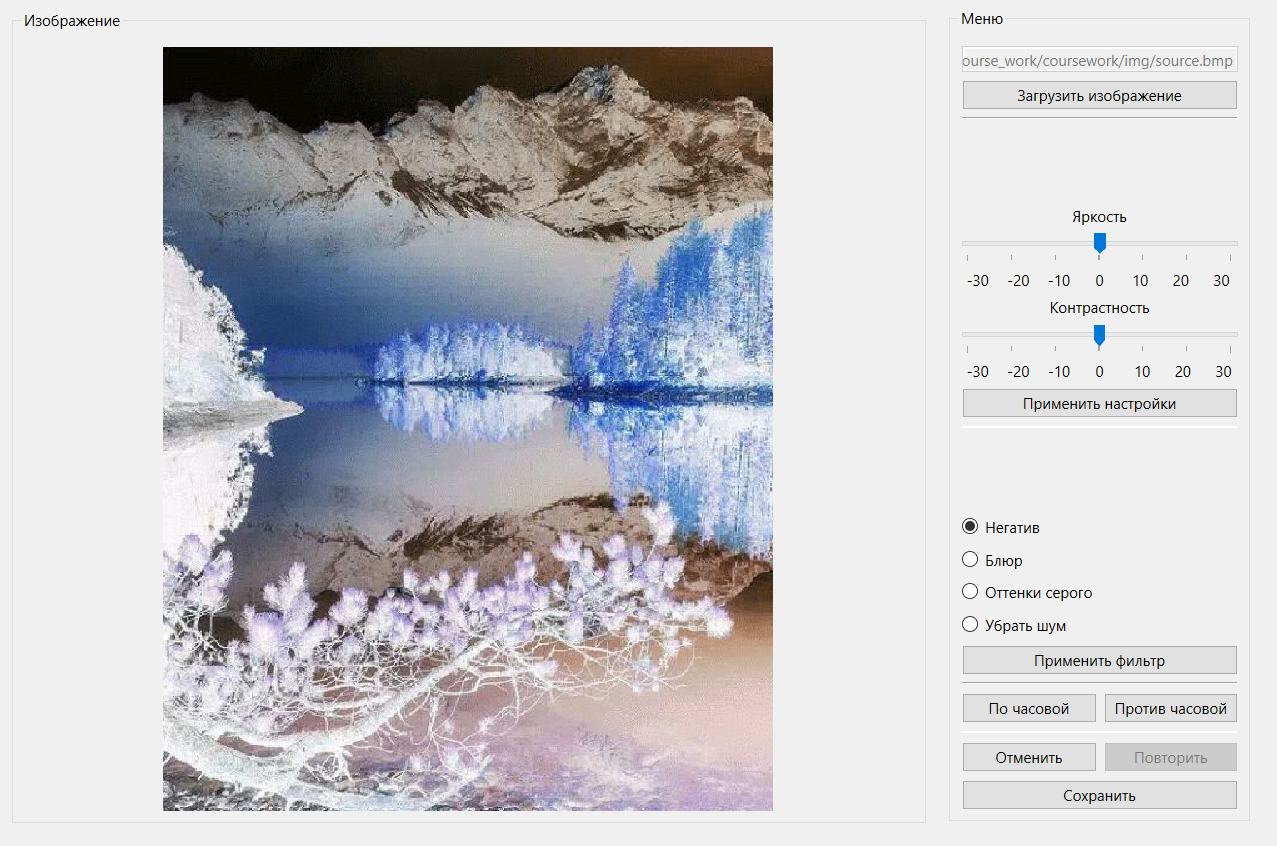
\includegraphics[width=0.7\textwidth]{img/res2.png}
	\caption{\label{fig:spire32} Фильтр негатива}
\end{figure}

\begin{figure}[hbtp]
	\centering
	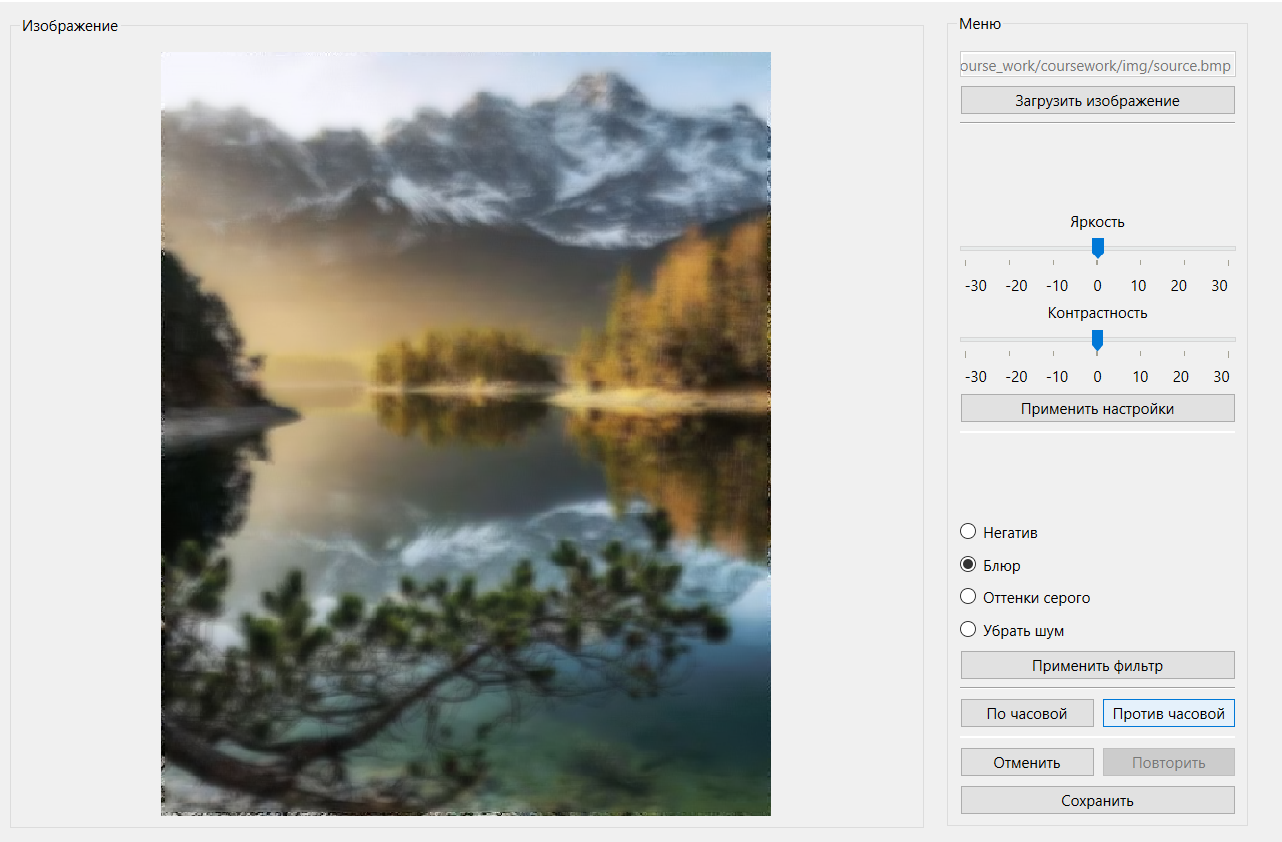
\includegraphics[width=0.7\textwidth]{img/res5.png}
	\caption{\label{fig:spire33} Фильтр размытия}
\end{figure}

\begin{figure}[hbtp]
	\centering
	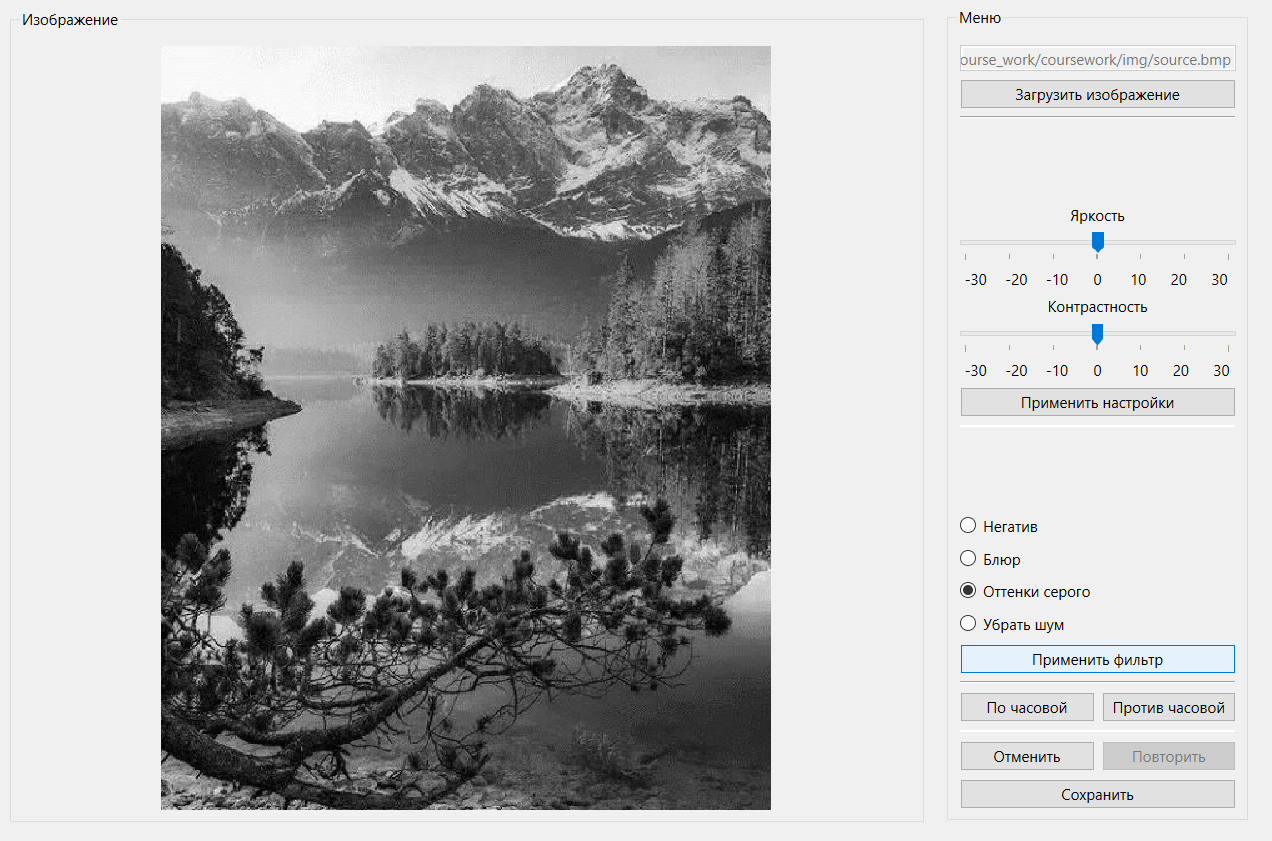
\includegraphics[width=0.7\textwidth]{img/res6.png}
	\caption{\label{fig:spire34} Фильтр оттенков серого}
\end{figure}

\begin{figure}[hbtp]
	\centering
	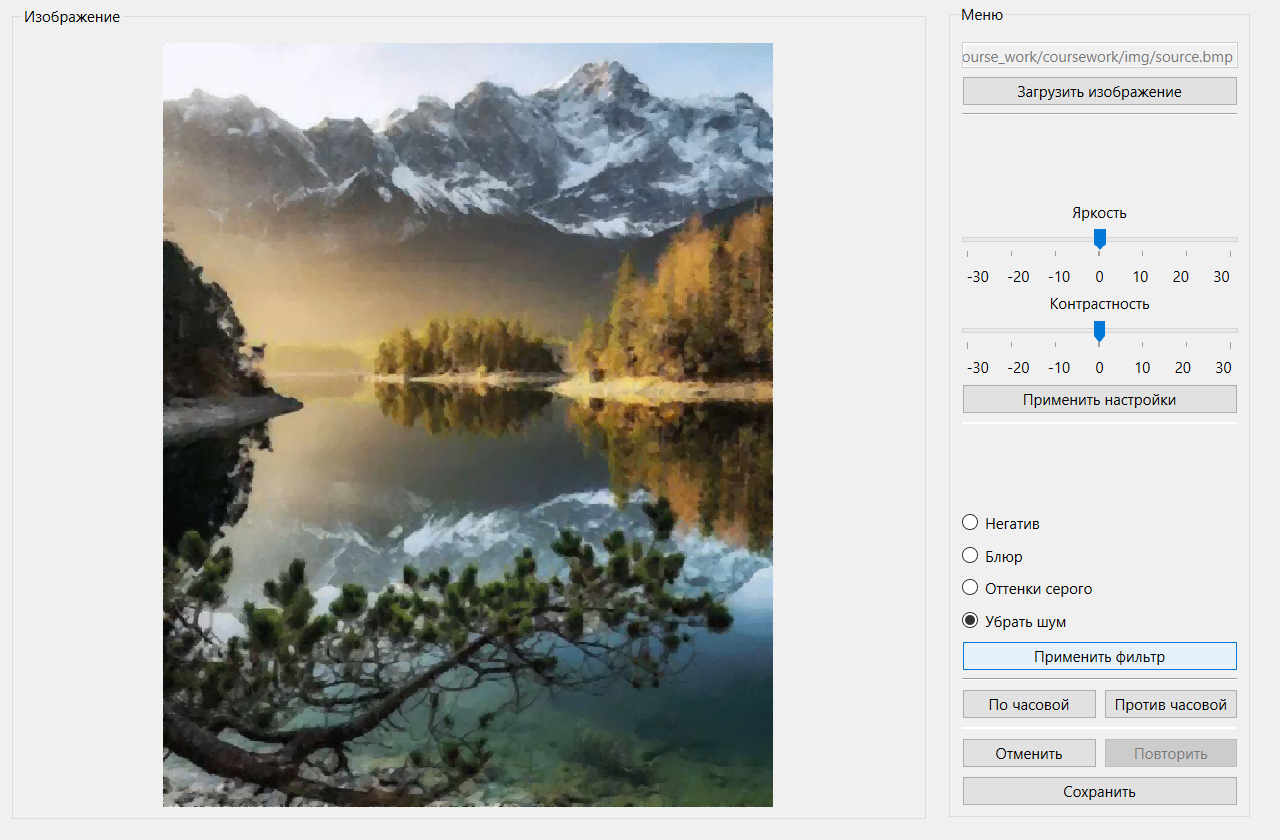
\includegraphics[width=0.7\textwidth]{img/res7.png}
	\caption{\label{fig:spire35} Фильтр уменьшения шума}
\end{figure}

Далее, на рисунках \ref{fig:spire36} и \ref{fig:spire37} представлены результаты изменения яркости, контрастности и поворота изображения последовательно.

\begin{figure}[hbtp]
	\centering
	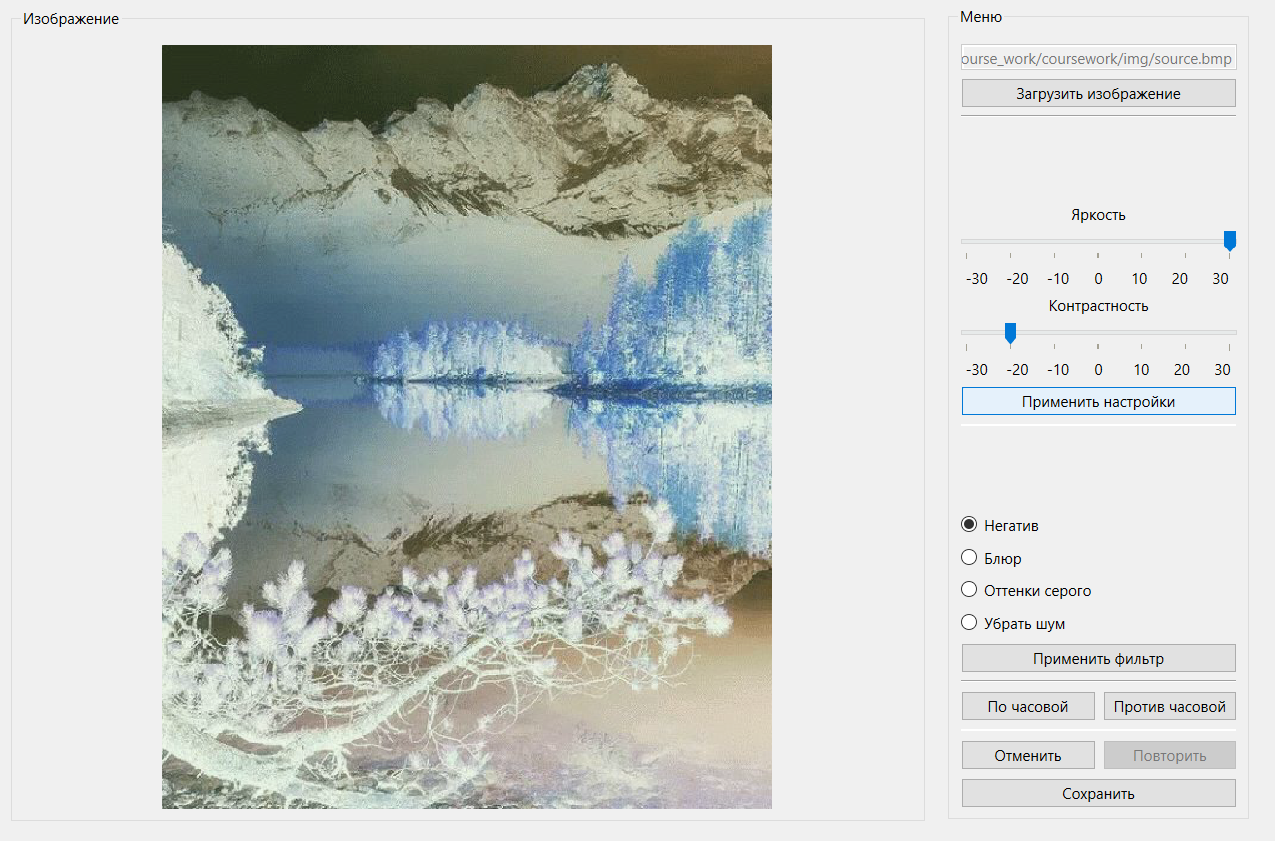
\includegraphics[width=0.7\textwidth]{img/res3.png}
	\caption{\label{fig:spire36} Изменение яркости и контрастности}
\end{figure}

\begin{figure}[hbtp]
	\centering
	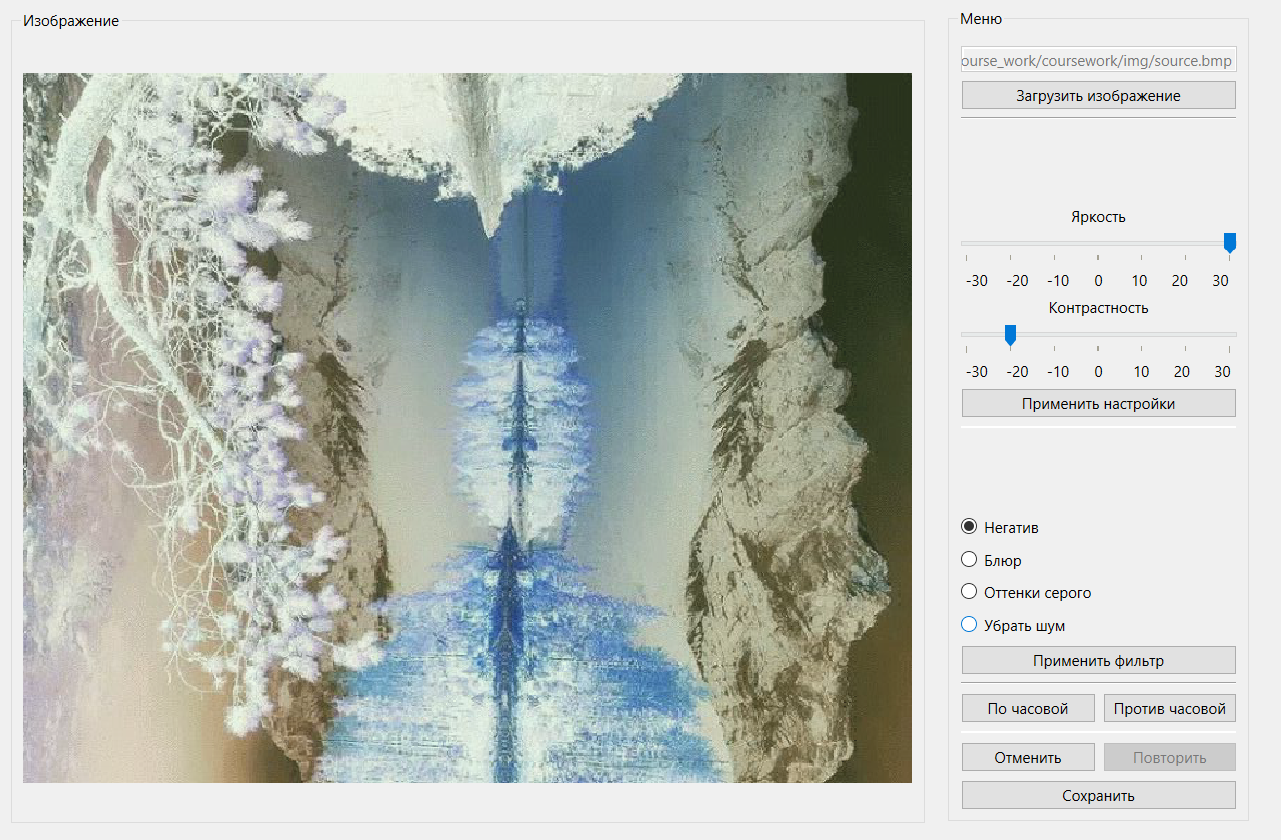
\includegraphics[width=0.7\textwidth]{img/res4.png}
	\caption{\label{fig:spire37} Поворот изображения}
\end{figure}

\clearpage

\subsection*{Выводы}

В данном разделе были рассмотрены детали реализации программного комплекса, представлены листинги кода алгоритмов обработки изображений и приведены примеры работы программы.

\pagebreak